\newpage

\section{overview}
In reinforcement learning we consider an \textit{agent} that collects \textit{reward} by acting in its \textit{environment}. The goal is to find a policy $\pi(a|s)$ that maps states to probability distributions over actions such that we get as much reward as possible. At time $t$ the state of the environment is $S_t \in \mathcal{S}$, and an agent can take an action $A_t \in \mathcal{A}(s)$. The environment then emits a reward $R_{t+1} \in \mathbb{R} $ and a subsequent state, $S_{t+1}$. Notice how the reward is just a scalar. From this sparse information the agent must learn to behave such that reward is maximized.

\begin{center}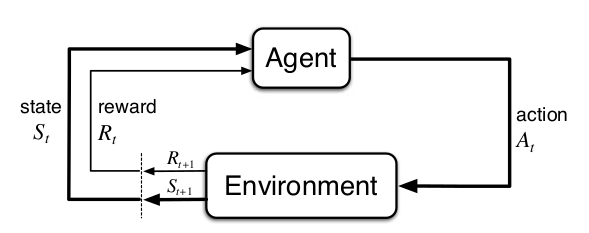
\includegraphics[width=.75\linewidth]{reinforcement_learning/agent_environment.png}\end{center}

The interactions between the agent, its actions, and the environment can be usefully modelled as Markov Decision Processes (MDPs). In Markov systems \textit{the future is independent of the past given the present}. The current state of the world tells you everything you need to know about what will happen next. Formally, $P(S_{t+1} \mid S_t) = P(S_{t+1} \mid S_0, S_1, \dots, S_{t})$. If the agent doesn't have complete information about the state of the world (i.e. it is \textit{partially observed}), a markovian environment can be non-markovian from the perspective of the agent.

Given a state $s$ and action $a$, the probability of moving to a new state $s'$ with reward $r$ is given by the following. Note that this maps four arguments to a single value, $p : \mathcal{S} \times \mathcal{S} \times \mathcal{A} \times \mathcal{R} \rightarrow [0,1]$.
$$ p(s', r | s, a) = Pr(S_t=s', R_t=r | S_{t-1}=s, A_{t-1}=a) $$
The function $ p(s', r | s, a) $ captures the dynamics of the environment. In model-based reinforcement learning we know (or learn) these dynamics, whereas in model-free methods we don't use them at all.

Our policy should not only encourage the acquisition of immediate reward, but also future reward. We therefore want to maximize \textit{returns}, which are a function of \textit{reward sequences}:

$$ G_t = R_{t+1} + R_{t+2} + \dots + R_{T}$$
This is an \textit{undiscounted return} because it equally weights all rewards. It is common to exponentially discount future rewards using a \textit{discount factor} $\gamma$ (animals exhibit similar temporal discounting):
$$
G_t = R_{t+1} + \gamma R_{t+2} + \gamma^2R_{t+3} + \dots = 
\sum_{k=0}^\infty \gamma^k R_{t+k+1}
$$
Note that we can define returns \textit{recursively}. Such recursive relationships are critical to many important ideas in reinforcement learning:
\begin{align*}
G_t &= R_{t+1} + \gamma R_{t+2} + \gamma^2R_{t+3} + \gamma^3R_{t+4} + \dots \\
&= R_{t+1} + \gamma(R_{t+2} + \gamma R_{t+3} + \gamma^2R_{t+4} +\dots) \\
&= R_{t+1} + \gamma G_{t+1}
\end{align*}
How can we maximize returns? A first thought might be to optimize the parameters of some policy with respect to the overall expected return (these are called \textit{policy gradient} methods). An alternative approach is to learn how good different states are. We can then maximize returns by selecting actions that move us to the best states.

A \textit{value function} captures how good different states are. Specifically, it tells us how much return we should expect in a given state:
\begin{align*}
v_\pi (s) &= \mathbb{E}[G_t \mid S_t=s] \\
&= \mathbb{E}[R_{t+1} + \gamma G_{t+1} \mid S_t=s] \\
&= \sum_a \pi (a|s) \sum_{s', r} p(s', r | s, a) [r + \gamma v_\pi (s')]
\end{align*}
Note that $R_t$ and $G_t$ are \textit{random variables}. The reward at a given time depends on the action select, $A_t \sim \pi (a \mid s)$, and the (potentially) stochastic environment dynamics, $R_t \sim p(s',r|s,a)$. Therefore, $\mathbb{E}[R_{t+1}] = \sum_a \pi (a|s) \sum_{s', r} p(s', r | s, a)r$.

The final line is a \textit{Bellman equation}, which recursively relates $v_\pi$ to itself. It says that the goodness of this state is the reward I expect immediately (averaging across all actions), plus the discounted goodness of the subsequent states (averaging across all subsequent states for each action). Notice that when we query the value of given state, we must consider all actions, subsequent states, and subsequent rewards, each weighted by their corresponding probabilities.

The value function $v_\pi(s)$ is a \textit{state-value} function because it reports the value of specific states. We will also consider \textit{action-value} functions, which report the value of state-action pairs.
\begin{align*}
q_\pi(s,a) &= \mathbb{E}[G_t | S_t=s, A_t=a] \\
&= \sum_{s',r} p(s', r | s, a) [r + \gamma v(s')] & \scriptstyle{\text{average over potential $s',r$}} \\
&= \sum_{s',r} p(s', r | s, a) [r + \gamma \sum_{a'} \pi(a' | s') q(s', a')] & \scriptstyle{\text{state-value is average over action-values}}
\end{align*}
The optimal policy $\pi_*$ yields the highest return for all states. The optimal state-value and action-value functions are denoted $v_*$ and $q_*$, respectively. They can be recursively defined using the \textit{Bellman optimality equations}:


\begin{align*}
v_*(s) &= \max_\pi v_\pi(s) \\
&= \max_a \sum_{s', r} p(s',r | s,a) [r + \gamma v_*(s')] \\
q_*(s,a) &= \max_\pi q_\pi(s,a) \\
&= \sum_{s', r} p(s',r | s,a) [r + \gamma \max_{a'} q_*(s', a')] \\
\end{align*}
This says that if our policy is optimal, we will always select actions that get us to the best possible subsequent state.

Many of these formulas can be intuited by drawing \textit{backup diagrams}. In backup diagrams, states are open circles and actions are black dots. The transitions from states (circles) to actions (dots) are governed by the policy $\pi(a \mid s)$. The transitions from actions (dots) to subsequent states (circles) are governed by the environment dynamics $p(s',r \mid s,a)$. 

Note that for $v_*$ we only consider the action with the maximum return (maximizing denoted by the arc symbol). Also note that each action can result in several possible states and rewards; this is why we need to average over these branches. Similarly, for $q_*$ we already know the state and action, but we must average over the potential states an rewards resulting from that action, followed by taking the action that maximizes our subsequent $q_*$ value.

\begin{center}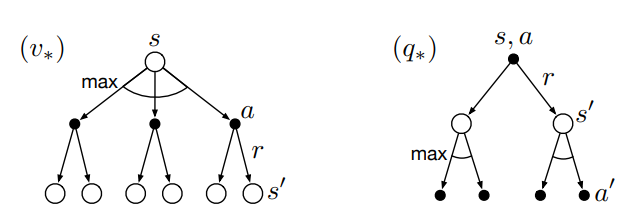
\includegraphics[width=.75\linewidth]{reinforcement_learning/backup_diagrams.png}\end{center}

\section{dynamic programming}
We usually don't have complete access to the state of the world and its dynamics. When we do, \textit{dynamic programming} can be used to iteratively converge on optimal policies. Generally, dynamic programming refers to algorithms in which a problem is decomposed into solvable sub-problems. If the same sub-problem is repeatedly encountered we can cache and re-use the solution.

The Bellman equations define a recursive relationship for value functions. We can therefore \textit{bootstrap}, using the solution of a previous problem (figuring out the value of $S_{t+1}$) to solve our current problem (figuring out the value of $S_{t}$). Using this logic, we will turn the Bellman equations into recursive update rules to converge on accurate value functions that can then be used to construct optimal policies.

Let's begin with \textit{policy evaluation}, or \textit{prediction}. This is the process of accurately determining the correct value function \textit{for a particular policy}. We are not improving our policy yet; rather, we are trying to figure out how good each state is under the current policy. To do this we take the Bellman equation for $v_\pi$ and turn it into a rule that updates $v_k$ to $v_{k+1}$:
\begin{align*}
v_{k+1}(s) &= \mathbb{E}[R_{t+1} + \gamma v(S_{t+1}) | S_t = s] \\
&= \sum_a \pi(a|s) \sum_{s',r} p(s',r|s,a) [r + \gamma v_k(s')]
\end{align*}
Keep in mind that this approach is biased. We are using an (initially) inaccurate estimate of subsequent states to update the value of the current state. Nonetheless, repeatedly applying this update (by repeatedly looping over all states) causes our estimate of the value function to converge on the true value function. 

Once we have an accurate value function we can update the policy by \textit{acting greedily with respect to it}. For example, if our policy says go left, but our value function says going right leads to a better state, we update our policy accordingly. 

But this leads to a problem. Our value function was defined with respect to $\pi_t$, but now we've updated the policy to $\pi_{t+1}$, which means our value function is no longer accurate! We therefore need to go back and update our value function again. We can then repeat the process of updating our value function and then our policy until we converge on an optimal policy. The algorithm is:
\begin{center}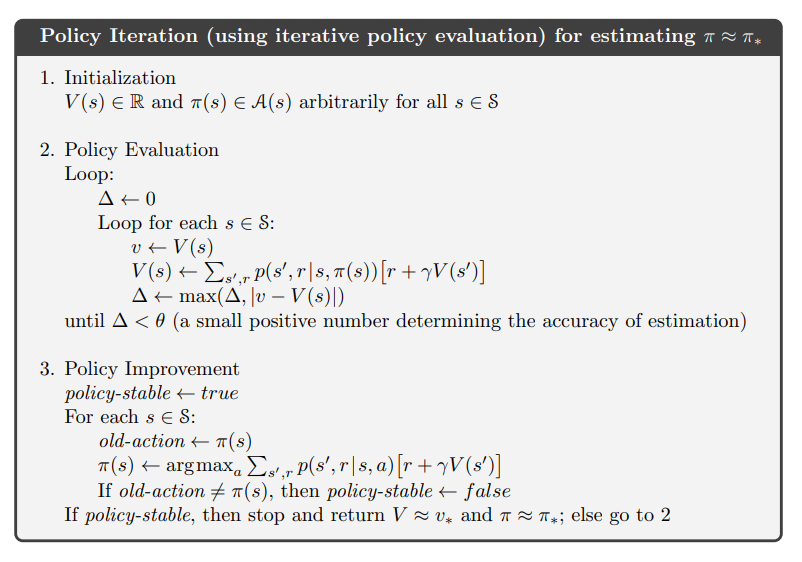
\includegraphics[width=.9\linewidth]{reinforcement_learning/policy_iteration.png}\end{center}

\subsection{value iteration}
As described above, after every policy improvement we need to iteratively improve our value function. How long do we need to iteratively improve the value function for a given policy? It turns out that even an imperfect but improved value function can help us improve the policy. In the extreme, we can update our value function with only a \textit{single} iteration, and always act greedily with respect to that value function. This is called \textit{value iteration}. It changes the problem, such that we are always working in value space and we ignore the policy until the very end, at which point the policy simply acts greedily with respect to the final value function. The update rule is:
$$
v_{k+1}(s) = \max_a \sum_{s',r} p(s',r|s,a) [r + \gamma v_k(s')]
$$
Notice that the value function takes the max rather than the expectation across actions. This means the value function only cares about the best possible action we could take in a given state. The algorithm is:

\begin{center}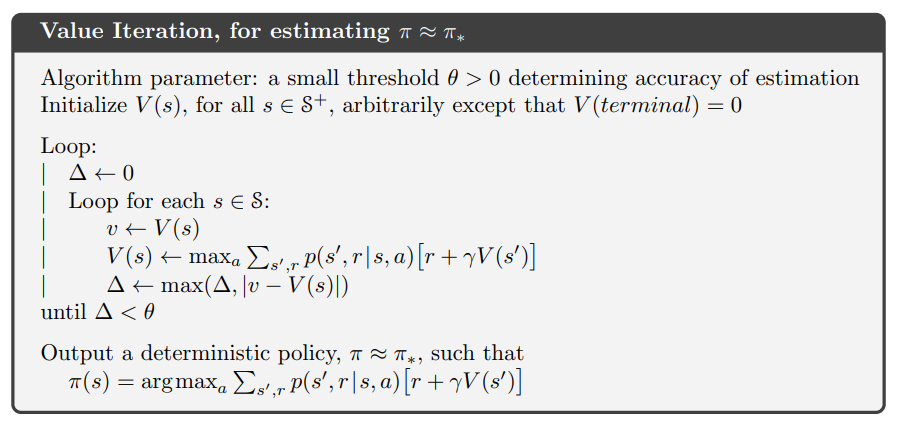
\includegraphics[width=.9\linewidth]{reinforcement_learning/value_iteration.png}\end{center}

In the algorithms presented above we sweep through all of the states to update our value function. But we could also perform these sweeps asynchronously or on-line, updating states that are actually visited by an agent. Critically, dynamically programming requires a perfect model of the dynamics of the world, which is usually not available!

\subsection{generalized policy iteration}
Many reinforcement learning algorithms can framed in a \textit{generalized policy iteration} framework, wherein we bounce back and forth between optimizing our policy and our value function:

\begin{center}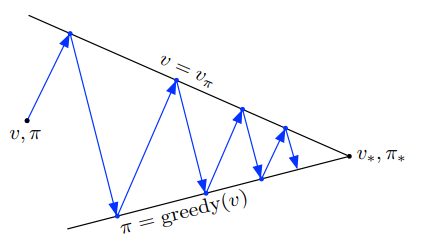
\includegraphics[width=.5\linewidth]{reinforcement_learning/gpi.png}\end{center}

\section{monte carlo methods}
Dynamic programming requires an accurate model of the environment; for every state-action pair we need to know the probability distribution over subsequent state-reward pairs, $p(s',r|s,a)$. Welcome to the real world, whose dynamics are usually unknown.

Whereas dynamic programming estimates values by averaging across all actions and subsequent states, \textit{monte carlo} methods use a simpler strategy: average the returns from a bunch of samples. These estimates will be correct on average (no bias), and with enough samples they will be quite accurate. We can then do control by acting greedy with respect to our value function.

\subsection{prediction}
Here is a simple algorithm for Monte Carlo \textit{prediction} (estimating $v_\pi(s)$ as opposed to optimizing $\pi$):

\begin{center}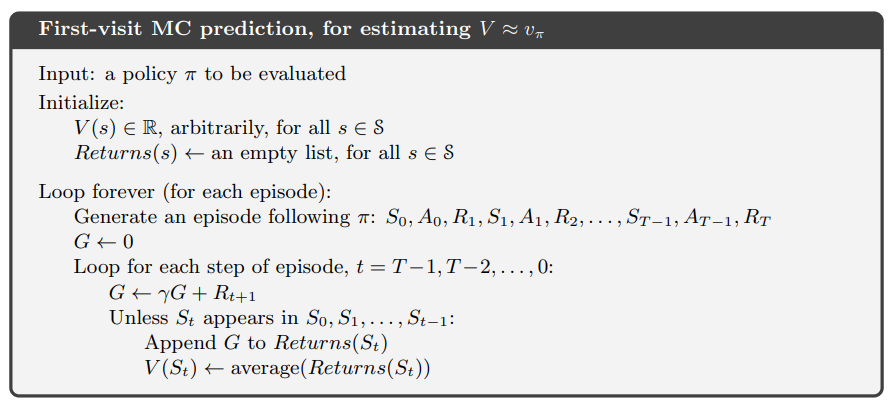
\includegraphics[width=.9\linewidth]{reinforcement_learning/mc_prediction.png}\end{center}

The annoying thing about monte carlo methods is that we need \textit{full trajectories} in order to update our value function for a state. The return at $t$ depends on all subsequent rewards until the end of an episode. We therefore can't update things online.

Therefore, in this algorithm we must start at the \textit{end} of a trajectory and move backwards, updating the value function only if we see a state that is the \textit{first visit} to that state during the trajectory (this contrasts with \textit{every visit} methods, which update the value function with every visit to a state in the trajectory).

\subsection{encouraging exploration}
In dynamic programming we looped over all states to update our value function. In monte carlo methods we generate data by actually rolling out our policy. This is nice because updates to the value function will focus on states that are actually relevant to our policy. However, we run the risk of insufficient \textit{exploration}.

How can we ensure that our agent sees potentially valuable states that are not visited under the current policy? One simple solution is with \textit{exploring starts}, in which we randomly choose the initial state and action.

Alternatively, we can learn stochastic policies that have a non-zero probability of selecting all available actions in all states. $\epsilon$\textit{-greedy} policies select the estimated best action with probability $(1-\epsilon)$ and a random action with probability $\epsilon$. Equivalently, the non-greedy actions have probability $\frac{\epsilon}{|\mathcal{A(s)}|}$, whereas the greedy action has the remainder of the probability, $1 - \epsilon + \frac{\epsilon}{|\mathcal{A(s)}|}$. $\epsilon$\textit{-soft} policies are a little 'fuzzier', and assign probabilities $\pi(a|s) \geq \frac{\epsilon}{|\mathcal{A(s)}|}$ for all states and actions:

\begin{center}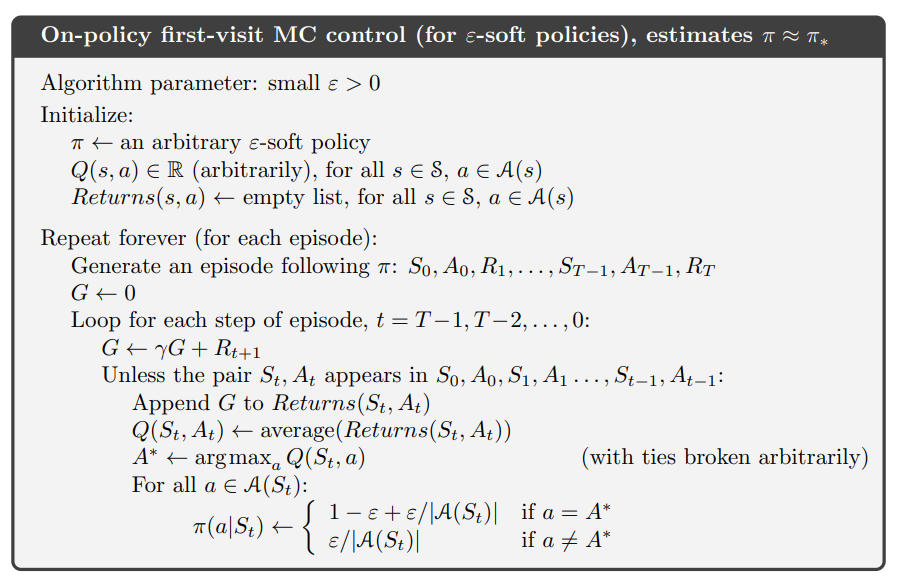
\includegraphics[width=.9\linewidth]{reinforcement_learning/mc_epsilon_soft.png}\end{center}

\subsection{off-policy prediction}
A very powerful way to ensure that the state space is adequately explored is to have separate \textit{behavior} and \textit{target} policies. The behavior policy guides behavior during data acquisition whereas the target policy is actually being evaluated. This allows us to explore the value of states that are unlikely to be visited under the target policy.

There's an important catch: if we sample trajectories under the behavior policy, we will estimate expected returns under the behavior policy, whereas we want to evaluate the target policy. To address this, we can weight each observed return by its likelihood under target policy relative to the behavior policy:
$$\rho_{t:T-1} = \prod_{k=t}^{T-1}\frac{\pi(A_k|S_k)}{b(A_k|S_k)}$$
Here $b$ is the behavior policy and $\rho_{t:T-1}$ is the weight associated with the trajectory occurring between times $t$ and $T-1$. By weighting the returns in this way, the expected value is the true value of the state under the target policy.

\textit{Ordinary importance sampling} estimates the value of a state by averaging weighted returns across all visits to a state $s$. Here $\mathcal{T}(s)$ is the set of all times at which state $s$ was visited and $T(s)$ is the time at which the episode containing time $t$ terminates.
$$V(s) = \frac{\sum_{t \in \mathcal{T}(s)} \rho_{t:T(t)-1} G_t}    {|\mathcal{T}(s)|}$$
This approach how no bias (it will converge to the desired expected value) but has very high variance. For example, if $\rho$ is large it can drastically overweight some returns. An alternative approach called \textit{weighted importance sampling} uses a weighted average, which results in much lower variance at the expense of higher bias:

$$V(s) = \frac{\sum_{t \in \mathcal{T}(s)} \rho_{t:T(t)-1} G_t}    {\sum_{t \in \mathcal{T}(s)} \rho_{t:T(t)-1}}$$
We can add control to this off-policy prediction method by acting greedily with respect to our action-value function:

\begin{center}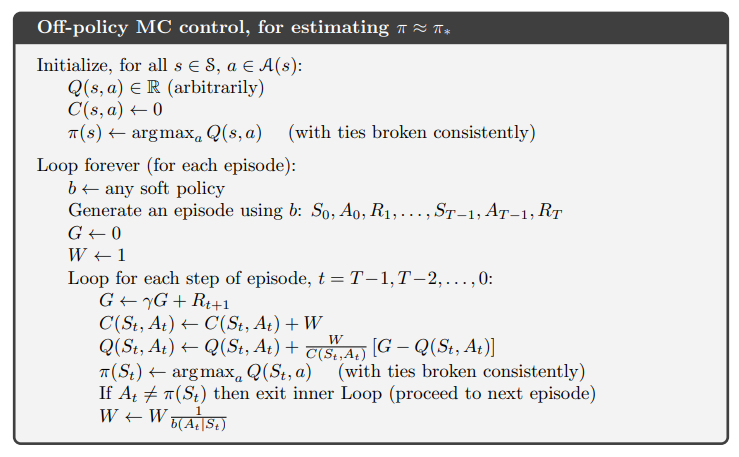
\includegraphics[width=.9\linewidth]{reinforcement_learning/mc_offpolicy.png}\end{center}


\section{temporal difference learning}
Temporal difference learning is a model free approach in which we sample (like monte carlo) \textit{and} bootstrap (like dynamic programming).

We update our value function by moving in the direction of the \textit{estimated} return. The returns are estimated ($R_t + \gamma V(S_{t+1})$) rather than directly observed ($G_t$). Whereas in Monte Carlo we updated $V(S_t) \leftarrow V(S_t) + \alpha [{\color{blue}G_t} - V(S_t)]$, now we update using:
\begin{align*}
V(S_t)
&\leftarrow V(S_t) + \alpha [{\color{blue}R_{t+1} + \gamma V(S_{t+1})} - V(S_t)] \\
&= V(S_t) + \alpha [{\color{blue}\delta_t} - V(S_t)]
\end{align*}

$\delta_t$ is the \textit{temporal difference error}, the difference between our bootstrapped estimate of the current return and our value estimate. TD learning has the advantage of being online; we don't have to wait until the end of our episode to update our value function. Furthermore, it reduces variance at the expense of increased bias (resulting from the value function initialization).

Monte Carlo and TD both converge to the true value function over time, but iteratively applying these methods to the same data reveals they are optimizing different things. Whereas Monte Carlo minimizes the mean squared error on the training data, TD finds the maximum-likelihood model for the underlying Markov process.

To illustrate, consider these sequences of states and rewards:
\begin{center}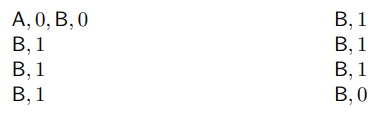
\includegraphics[width=.4\linewidth]{reinforcement_learning/td_series.png}\end{center}

Monte Carlo gives a value of 0 to A, because every time we saw A there was a return of 0. However, (undiscounted) TD learning gives A a value of $\frac{6}{8}$, because A is always been followed by B, which itself has a value of $\frac{6}{8}$. TD has learned the maximum-likelihood MDP with the following structure:

\begin{center}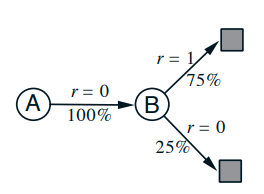
\includegraphics[width=.3\linewidth]{reinforcement_learning/td_series_model.png}\end{center}

\subsection{SARSA}

\begin{wrapfigure}{r}{.075\linewidth}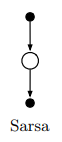
\includegraphics[width=1\linewidth]{reinforcement_learning/backup_sarsa.PNG}\end{wrapfigure}

SARSA learns action-value functions using an update rule analogous to the state-value update rule described above. Given a \textbf{S}tate, we select an \textbf{A}ction, observe the \textbf{R}eward / subsequent \textbf{S}tate, and then bootstrap our action-value function using our policy to select the next \textbf{A}ction:
$$  Q(S_t, A_t) \leftarrow Q(S_t, A_t) + \alpha [R_{t+1}  + \gamma Q(S_{t+1}, A_{t+1}) - Q(S_t, A_t)]  $$

\subsection{Q-learning}

\begin{wrapfigure}{r}{.1\linewidth}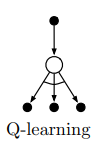
\includegraphics[width=1\linewidth]{reinforcement_learning/backup_qlearning.PNG}\end{wrapfigure}

SARSA learns the action-value function associated with a given policy. The policy can then be improved by acting greedily with respect $q$. \textit{Q-learning} is an off-policy algorithm that directly approximate $q_*$. To do this, we take the best action when bootstrapping, as opposed to the action chosen by our current policy:
$$  Q(S_t, A_t) \leftarrow Q(S_t, A_t) + \alpha [R_{t+1}  + \gamma \max_a Q(S_{t+1}, a) - Q(S_t, A_t)]  $$
\subsection{expected SARSA}

\begin{wrapfigure}{r}{.15 \linewidth}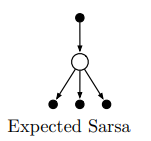
\includegraphics[width=1\linewidth]{reinforcement_learning/backup_expectedsarsa.PNG}\end{wrapfigure}

In SARSA, $A_{t+1}$ is a random variable that is selected according to our policy. This randomness introduces variance that can be mitigated by taking the expectation of subsequent actions:

$$  Q(S_t, A_t) \leftarrow Q(S_t, A_t) + \alpha [R_{t+1}  + \gamma \sum_a \pi(a|S_{t+1}) Q(S_{t+1}, a) - Q(S_t, A_t)]  $$

\section{n-step bootstrapping}
In Monte Carlo we sample entire trajectories. This method is low bias but has high variance due to sampling error. In TD(0) we sample one step and then bootstrap on our value function. This method has bias but much lower variance.

Although these approaches may appear qualitatively different, they are in fact the extremes of a continuum. In general we can take $n$ steps and then bootstrap. The number of steps determines the bias-variance trade-off (bigger $n \rightarrow$ less bias, more variance):

\begin{center}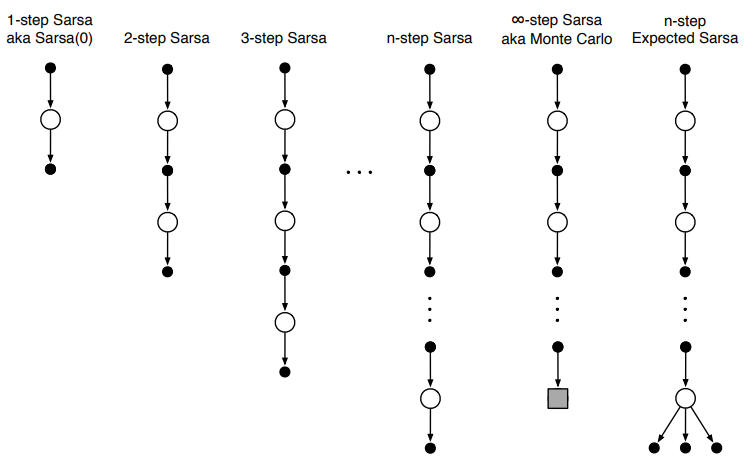
\includegraphics[width=.7\linewidth]{reinforcement_learning/nstep.png}\end{center}

The $n$ step return and its associated update rule (for state-value functions) are:
\begin{gather*}
G_{t:t+n} = R_{t+1} + \gamma  R_{t+2} + \gamma^2  R_{t+3} + \dots + \gamma^{n-1}  R_{t+n} + V(S_{t+n}) \\ \\
V(S_t) \leftarrow V(S_t) + \alpha [G_{t:t+n} - V(S_t)]
\end{gather*}

Intuitively, taking larger $n$ allows us to see further back when assigning credit/blame to states and actions that led to reward. For example, upon reaching a reward state in TD(0) we only updated the value of the states/actions that caused reward, but the actions \textit{that led to} the actions that caused reward are not updated. With $n=10$, however, we can assign credit to several states in the sequence that resulted in reward:

\begin{center}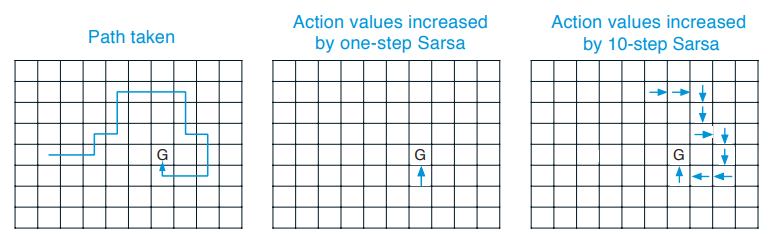
\includegraphics[width=.8\linewidth]{reinforcement_learning/nstep_paths.png}\end{center}

\section{the big picture}
\subsection{breadth vs. depth}
The methods we've applied so far vary in breadth and depth. Methods that bootstrap (DP and TD) are shallow in that they only step a little into the future before bootstrapping. Monte Carlo is deep in that it samples until the end of trajectories. Furthermore, methods that take expectations over actions are wide, such as DP, whereas both TD and Monte Carlo can be thought of as narrow because they rely on sampling rather than averaging over actions. 

Methods exist in between these extremes and can be thought of as living in a space characterized by two axes. These axes represent the extent to which a method relies on sampling vs. expectations (narrow vs. wide), and bootstrapping vs. sampling (shallow vs. deep): 

\begin{center}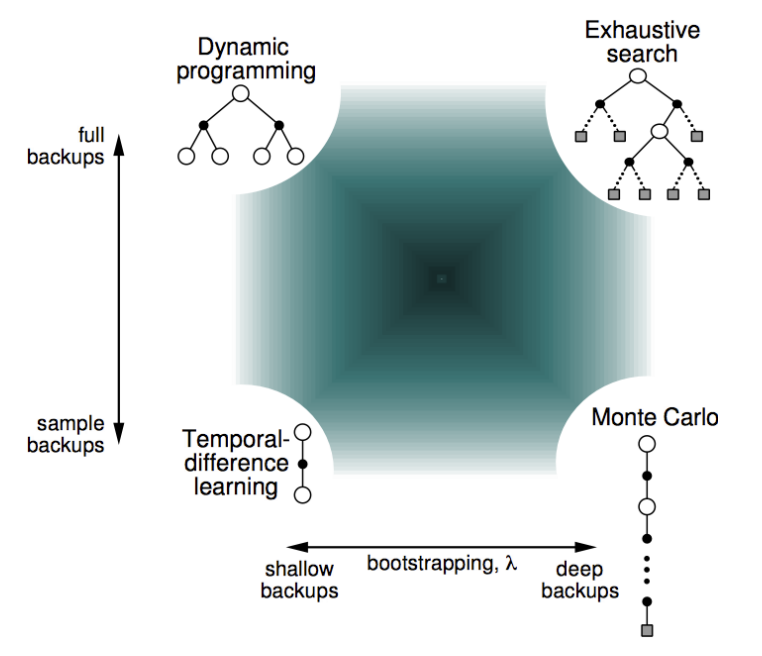
\includegraphics[width=.6\linewidth]{reinforcement_learning/rl_bigpicture.PNG}\end{center}

\subsection{value function updates}
The value function updates we've considered differ in whether they 1) update the state or action value function, 2) approximate the optimal or an arbitrary policy, and 3) rely on sample or expected updates. The different combinations of these three binary dimensions yield the following family of value function updates: 

\begin{center}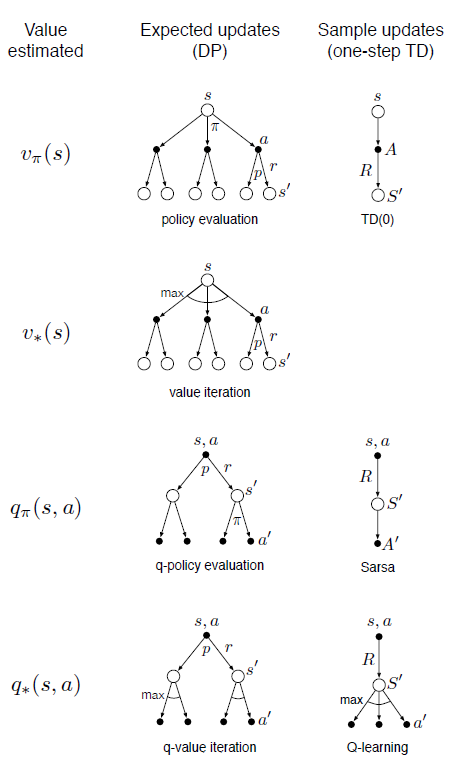
\includegraphics[width=.5\linewidth]{reinforcement_learning/value_updates.PNG}\end{center}

\section{learning your model}
Thus far we have discussed model-free algorithms and algorithms that require a model of the world, $p(s',r \mid a,a)$, such as dynamic programming. When utilizing models we can distinguish between \textit{real} and \textit{simulated} experience. Real experience results from interactions with the world (e.g. observing the consequences of taking action $a$ in state $s$), whereas simulated experience results from querying the model (e.g. the model predicts what would happen if the agent were to take action $a$ in state $s$). There is a related distinction between \textit{planning} and \textit{learning}. Planning uses a model (simulated experience) to find better actions, whereas learning relies upon real experience with the environment.

We can also consider algorithms that \textit{learn} a model of the world through experience. For such algorithms, the utility of real experience is two-fold: it can be used to update the value function (\textit{direct reinforcement learning}) in addition to improving the model (\textit{model learning}):

\begin{center}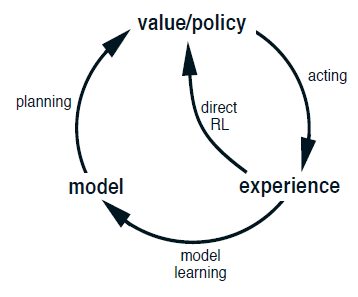
\includegraphics[width=.4\linewidth]{reinforcement_learning/planning_learning.PNG}\end{center}

\subsection{DynaQ}
DynaQ is a simple algorithm that utilizes both planning and learning. The agent takes actions (b,c), updates the value function based on the observed reward via Q-learning (direct RL; d), updates the model of the world based on that experience (using a simple lookup table in this example; e), then uses the model to generate simulated experience that further refines the value function (f):

\begin{center}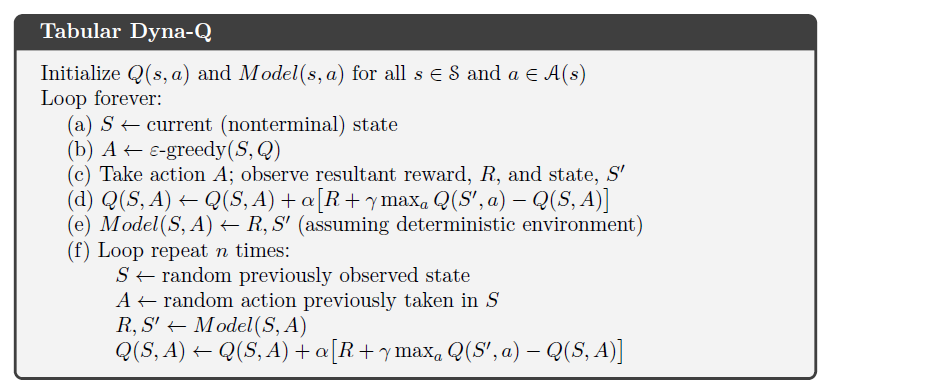
\includegraphics[width=1\linewidth]{reinforcement_learning/dynaq.PNG}\end{center}

\section{smarter state updates}
In the dynamic programming algorithms discussed previously we updated the value function by looping over and updating all states (or state-action pairs). However, states with very low value may be seldom/never visited under our policy. We may therefore benefit by focusing our updates on more important states.

\subsection{prioritized sweeping}
If an agent encounters a state which causes a large change in the value function (e.g. the state had a much higher or lower return than expected), we update this state accordingly. However, we should also update states that \textit{led} to that state.

Prioritized sweeping accomplishes this by maintaining a queue of state-actions for which there is a high change in the value function, sorted by the magnitude of that change. After every step in the environment, we loop through queue. For each state-action, we update the value function \textit{and then loop through all state-actions predicted by the model to lead to that state}. Many of these state-actions will also have high return changes because they lead to a state with a high change. These state-actions are also added to the cue and the process is repeated until the queue is depleted.

\subsection{trajectory sampling}
Rather than sweeping across all states, we can sample states according to how likely they are to be visited under the current policy. Although we don't know this distribution explicitly, we can approximate it by simply letting the agent interact with the world according to the policy, and update states/actions that are visited during these trajectories. Such \textit{trajectory sampling} paired with the value-iteration dynamic programming algorithm results in \textit{real-time dynamic programming}.

\section{decision-time planning}
In decision-time planning we explore a tree of possible outcomes resulting from different actions we could take at every state we reach. In \textit{heuristic search} we can estimate the value of an action by taking the action, following a policy for a certain number of steps, and then bootstrapping on the value function at leaf nodes (this requires a model that we can use to generate these simulated trajectories). In \textit{rollout algorithms} we use a monte carlo approach to estimate the value of each action, e.g. by taking that action many times and averaging the returns. \textit{Monte carlo tree search} extends this idea by focusing on sub-trajectories that have higher estimated values, and extending the search tree selectiviely in these directions. This strategy was critical for the famous AlphaGo algorithm.

\section{value function approximation}
The tabular methods we have discussed thus far are limited when the action and/or state spaces are very large, and impossible when they are continuous. Value function approximation solves both problems by using a function to approximate the relationship between a representation of the state and the value of that state. A value function parameterized by weights $\mathbf{w}$ is denoted $\hat{v}(s, \mathbf{w})$.Note that there is a lot of flexibility in how we represent the state. In general, we will represent each state $s$ by a vector $\mathbf{x}(s)$.

\subsection{stochastic gradient descent}
We can learn the value function (i.e. its parameters $\mathbf{w}$) via gradient descent. This requires defining a loss functions and taking its gradient $\nabla$ with respect to $\mathbf{w}$. We will compute the mean squared error between the estimated and true value function, averaged across states with weights $u(s)$ ($\mu(s)$ is typically the \textit{stationary distribution} of states under the current policy):
$$
\overline{VE}(\mathbf{w}) = \sum_{s \in \mathcal{S}} u(s) \left[v_\pi(s) - \hat{v}_\pi(s, \mathbf{w})\right]^2
$$
We can make our value estimate more accurate by nudging $\mathbf{w}$ in the direction of the gradient. Because the states should be distributed according to $u(s)$, the expectation for these updates should be the true update. Recall that the gradient is a vector describing how each variable in a scalar valued function affects the output: $\nabla_\mathbf{w} f(\mathbf{w}) = \left( \frac{\partial f(\mathbf{w})}{\partial w_1}, \frac{\partial f(\mathbf{w})}{\partial w_2}, \dots, \frac{\partial f(\mathbf{w})}{\partial w_d} \right)^\top$. We will oftentimes omit the subscript in $\nabla_\mathbf{w}$.

Our stochastic gradient ascent algorithm will nudge $\mathbf{w}$ in the direction of the gradient for each $S_t$ we observe:
\begin{align*}
\mathbf{w_{t+1}} &= \mathbf{w_{t}} + \alpha \frac{1}{2} \nabla \left[v_\pi(s) - \hat{v}_\pi(S_t, \mathbf{w})\right]^2 \\
&= \mathbf{w_{t}} + \alpha \left[{v_\pi(S_{t})} - \hat{v}_\pi(S_t, \mathbf{w})\right] \nabla \hat{v}_\pi(S_t, \mathbf{w}) & \scriptstyle{\text{chain rule}}
\end{align*}
So far so good, but if we knew $v_\pi(s)$ we wouldn't need to be reading this book! Instead we use a \textit{target} to approximate $v_\pi(s)$. If the target is a real return, $G_t$, the updates will be unbiased because the value function is the expectation over returns. A gradient monte carlo algorithm therefore updates the weights according to:
$$ \mathbf{w_{t+1}} = \mathbf{w_{t}} + \alpha \left[{\color{blue}G_t} - \hat{v}_\pi(S_t, \mathbf{w})\right] \nabla \hat{v}_\pi(S_t, \mathbf{w}) $$
We could alternatively use a TD(0) target :
$$ \mathbf{w_{t+1}} = \mathbf{w_{t}} + \alpha \left[{\color{blue}R_t + \gamma \hat{v}_\pi(S_{t+1}, \mathbf{w})} - \hat{v}_\pi(S_t, \mathbf{w})\right] \nabla \hat{v}_\pi(S_t, \mathbf{w}) $$
There's a subtlety here: when we took the gradient above, the original target $v_\pi(s)$ did not depend on $\mathbf{w}$. But our esimated target, $\hat{v}(s, \mathbf{w})$, depends on $\mathbf{w}$. Using a bootstrapped target containing our estimated value function invalidates the math. This approach is therefore called \textit{semi-gradient}. It still works in practice, but at the expense of some theoretical guarantees.

\subsection{state representations}
Imagine a task in which the true dimensionality of the state space is $\mathbb{R}^2$. In mountain car, for example, the state is simply the position and velocity of the car. In this case the true value function (for the optimal policy) can be visualized as a surface in $\mathbb{R}^2$, and it is quite complex:
\begin{center}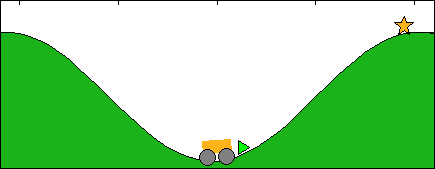
\includegraphics[width=.4\linewidth]{reinforcement_learning/mountaincar.PNG}\end{center}
\begin{center}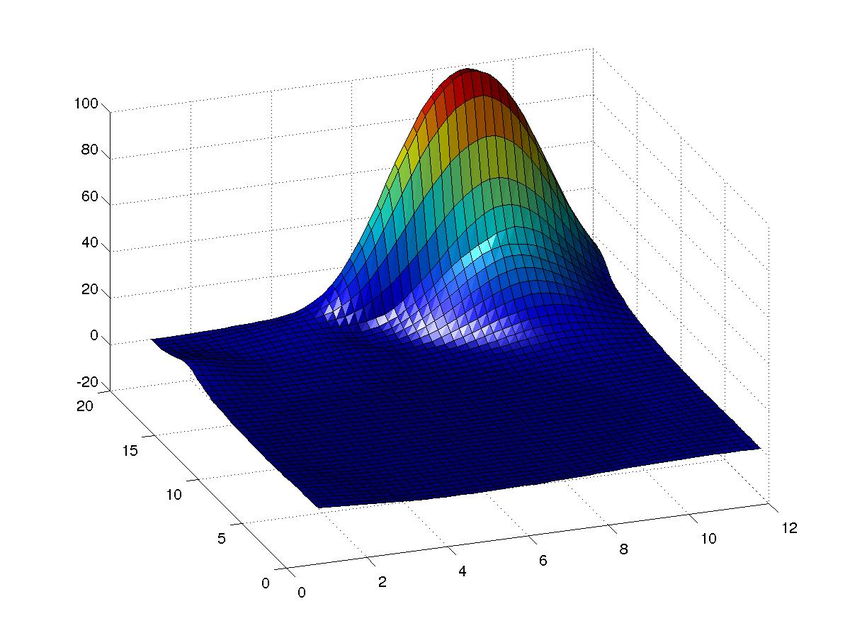
\includegraphics[width=.4\linewidth]{reinforcement_learning/mountaincar_value.PNG}\end{center}

Now consider a linear value function that takes a weighted sum of the state representation, $\hat{v}(s, \mathbf{w}) = \mathbf{w}^\top \mathbf{x}(s)$. If $\mathbf{x}(s)$ is just a vector containing the position and velocity, then we could only create planar value functions that intersect the origin. We could fix this by making the value function more complex, e.g. a neural network. An alternative solution is to build a state representation $\mathbf{x}(s)$ that allows more complex value functions to be constructed.

\textit{Polynomials}. In polynomial bases, each element $x_i(s)$ is a product of some combination the original elements raised to some power. For example, if the position and velocity in mountain car are $(s_1, s_2)$, then we could have $\mathbf{x}(s) = (1, s_1, s_2, s_1s_2, s_1^2s_2, s_1s_2^2,s_1^2s_2^2)$. Now we can create more complex value function surfaces in $\mathbb{R}^2$.

\textit{Fourier basis.} Periodic (well-behaved) functions of arbitrary complexity can be represented as a sum of trigonometric functions. Using this logic, we can create state representations where each element is a trigonometric function of our original data with a characteristic frequency in each dimension: $x_i(s) = cos(\pi \mathbf{s}^\top c_i)$. The elements of each $c_i$ control the frequency of each dimensions, as follows:
\begin{center}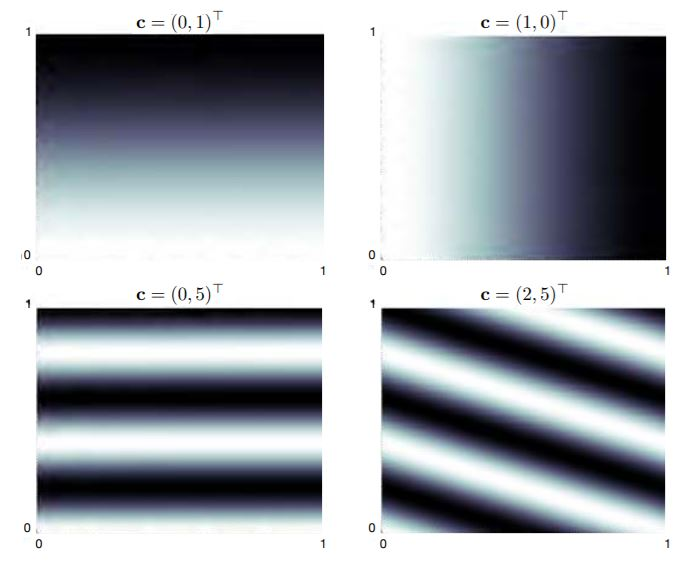
\includegraphics[width=.4\linewidth]{reinforcement_learning/fourier_basis.JPG}\end{center}

\textit{Tiling.} What if we just slice up our state space into a grid, with $\mathbf{x}(s)$ becoming a one-hot vector representation of our grid location? With a linear value function, this actually turns the problem back into a lookup table, with $\mathbf{w}$ now storing the estimated values of each state. This shows that function approximation is actually a generalization of the tabular case. We can be more clever though. If we have several grids, each offset from one another, then every point in the space will activate multiple, partially overlapping grid points.

\begin{center}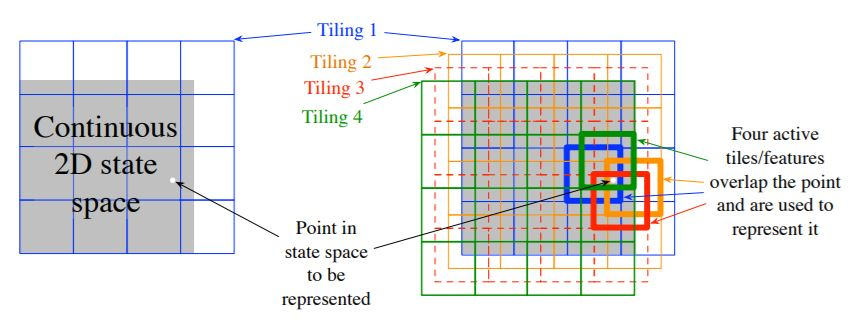
\includegraphics[width=.8\linewidth]{reinforcement_learning/tiling.JPG}\end{center}

Overlapping grids allow generalization to occur. We can also encourage generalization in particular dimensions/directions by creating longer rectangles or even full stripes that extend in the direction that generalization should occur.

\subsection{function approximators}
Anything differentiable can be used for $\hat{v}$, such as an artificial neural network or linear regression.

There are also non-parametric approaches to function approximation. For example, a nearest neighbors approach could take the mean of the $k$ visited states that are closest to the current state. Or we could take a mean across all visited states weighted by their closeness. Kernel methods use a function $k(s,s')$ that assigns a weight for each $s'$ when estimating the value of $s$: $\hat{v}(s,\mathbf{w}) = \sum_{s' \in \mathcal{D}} k(s,s') g(s')$. Here $g(s')$ is the target (e.g. return for monte carlo, bootstraped return for TD(0)) for the previously visited state $s'$.

\subsection{control with function approximation}
To use function approximation for control rather than prediction, we can learn an action-value function and follow a policy that acts greedily with respect to it. Following the pattern above, we can update our weights (for example by following a SARSA target) as:
$$
\mathbf{w_{t+1}} = \mathbf{w_{t}} + \alpha \left[{\color{blue}R_t + \gamma \hat{q}_\pi(S_{t+1}, A_{t+1}, \mathbf{w})} - \hat{q}_\pi(S_t, A_t, \mathbf{w})\right] \nabla \hat{v}_\pi(S_{t}, \mathbf{w})
$$
\section{differential returns}
Rather than considering rewards at each time step, we can ask how each reward differs from the average reward, $r(\pi)$, under our current policy. Differential returns are defined as:
$$
G_t = R_{t+1} - r(\pi) + R_{t+2} - r(\pi) + R_{t+3} - r(\pi) + \dots
$$
With differential returns we can avoid discounting in the continuous case, as there is no concern that the returns will explode. Differential returns can be used, for example, in Bellman equations and TD updates, as follows:
\begin{gather*}
v_\pi(s) = \sum_a \pi(a \mid s) \sum_{s',r} p(s',r \mid s, a) \left[r - r(\pi) + \gamma v_\pi(s') \right] \\
\delta_t = {\color{blue} R_{t+1} - \bar{R}_t + \hat{v}_\pi(S_{t+1}, \mathbf{w}_t)} - \hat{v}_\pi(S_t, \mathbf{w}_t)
\end{gather*}
$\bar{R}_t$ is our estimate of $r(\pi)$ at time $t$. Notice that we need to keep a running estimate of the average reward. By analogy to how we update value functions in TD methods, we might select the update rule $\bar{R}_{t+1} \leftarrow \bar{R}_t + \beta [R_{t+1} - \bar{R}_t]$. However, it turns out that using $\delta_t$ reduces the variance of our updates: $\bar{R}_{t+1} \leftarrow \bar{R}_t + \beta \delta_t$

\section{$\lambda$ return}
$n$-step returns ($G_{t:t+n}$) allow us to control the extent to which we rely on sampling (big $n$) vs. bootstrapping (small $n$). Rather than picking a single $n$, we can take take an exponentially weighted average of $n$-step returns for all $n$:
$$ G_t^\lambda = (1-\lambda) \sum_{n=1}^\infty \lambda^{n-1}G_{t:t+n} $$
$(1-\lambda)$ ensure the weights sum to 1. Note that for $\lambda=0$ this reduces to a one step return, whereas for $\lambda=1$ it is a monte carlo return. The weighting scheme is visualized as follows. Notice that all returns which reach the terminal state are collectively given the rest of the weight:

\begin{center}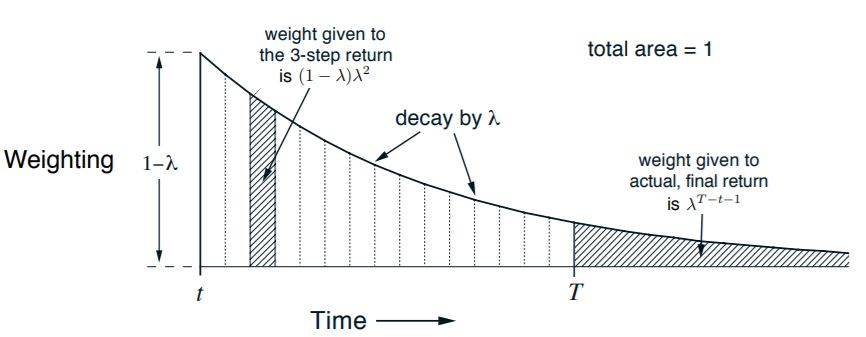
\includegraphics[width=.6\linewidth]{reinforcement_learning/lambda_return.JPG}\end{center}

For continuous settings we can't compute $n$-step returns for arbitrarily large $n$. We can therefore approximate $G_t^\lambda$ by taking the first $k$ returns. By setting all $G_{t:t+k+\delta} =G_{t:t+k} $ for $\delta \in \mathbb{N}$ we give all the residual weight to $G_{t:t+k}$:

\begin{align*}
G_{t:t+k}^\lambda
&= (1-\lambda) \sum_{n=1}^\infty \lambda^{n-1}G_{t:t+n} \\
&= (1-\lambda) \sum_{n=1}^{k-1} \lambda^{n-1}G_{t:t+n} + (1-\lambda) \sum_{n=k}^{\infty} \lambda^{n-1}G_{t:t+n} \\
&= (1-\lambda) \sum_{n=1}^{k-1} \lambda^{n-1}G_{t:t+n} + (1-\lambda) \sum_{n=k}^{\infty} \lambda^{n-1}G_{t:t+k} & \scriptstyle{\text{we are setting $G_{t:t+k+\delta} =G_{t:t+k} $ for $\delta \in \mathbb{N}$}}\\
&= (1-\lambda) \sum_{n=1}^{k-1} \lambda^{n-1}G_{t:t+n} + \lambda^{k-1}(1-\lambda) \sum_{n=1}^{\infty} \lambda^{n-1} G_{t:t+k} & \scriptstyle{\text{re-index and factor out $\lambda^{k-1}$}} \\
&= (1-\lambda) \sum_{n=1}^{k-1} \lambda^{n-1}G_{t:t+n} + \underbrace{\lambda^{k-1}G_{t:t+k}}_\text{residual weight} & \scriptstyle{\text{because $\sum_{n=1}^{\infty} \lambda^{n-1} = \frac{1}{1-\lambda}$}}
\end{align*}

\subsection{offline $\lambda$ return algorithm}
The \textit{offline $\lambda$ return algorithm} performs weight updates after each episode according to the $\lambda$ return at each time point using semi-gradient ascent as follows:
$$
\mathbf{w}_{t+1} = \mathbf{w}_t + \alpha \left[G_t^\lambda - \hat{v}(S_t, \mathbf{w}_t) \right] \nabla_\mathbf{w} \hat{v}(S_t, \mathbf{w}_t)
$$
\subsection{online $\lambda$ return algorithm}
We can perform truncated $\lambda$ return updates online, but this requires a trick. If we are interested in $5$-step $\lambda$ returns, but we are only at $t=2$, we start by computing the $2$ -step return. Then when $t=3$, we go back and update our previous weight updates using the most recently available returns, and so on.

\section{forward vs. backward views}
Value functions are expectations over returns, which are a function of \textit{future} rewards. Every time we encounter a state, we update it's value in the direction of immediate rewards, and to a lesser extent distant rewards. We continue moving state by state, associating rewards with states based on their temporal proximity.

If a reward occurs soon \textit{after} a state, we associate the reward with the state. By the same token, if a state occur soon \textit{before} a reward, we should make the same association. This \textit{backward view} is appealing because it opens the door to efficient, online algorithms for value function updates.

For the backward view to work, we need to keep track of how recently we visited each state. Just as rewards are discounted exponentially as time passes, our recency metric will fade exponentially. This recency metric is called as \textit{eligibility trace}, $\mathbf{z}$. If we have a one-hot vector representation of the state, $\mathbf{x}$, then when we visit state $s$ we have $x_s \leftarrow x_s+1$ and $x_{i} \leftarrow \gamma \lambda x_i $. For each $x_i$ this causes decay patterns like this:

\begin{center}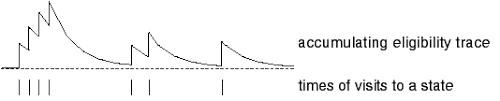
\includegraphics[width=.7\linewidth]{reinforcement_learning/trace_decay.png}\end{center}

\subsection{TD($\lambda$)}

TD($\lambda$) \textit{approximates} the offline $\lambda$-return using an efficient backward view algorithm. We first need to generalize eligibility traces to function approximation. Recall that the general formulation for weight updates is:
$$ \mathbf{w}_{t+1} = \mathbf{w}_t + \alpha \delta_t \nabla_\mathbf{w} \hat{v}(S_t, \mathbf{w}_t) $$
$\delta_t$ is the difference between the target and our current value estimate. This tells us how much we should be surprised by what is happening \textit{now}. The associated update rule for the eligibility trace is:
$$
\mathbf{z}_{t} = \gamma \lambda \mathbf{z}_{t-1} + \nabla \hat{v}(S_t, \mathbf{w}_{t})
$$
This more general eligibility trace no longer strictly reflects the recency of states. Rather, it reflects how elegible each element in $\mathbf{w}$ is for tweaking when something good or bad happens. It is like a smeared out version of the gradient. The new weight update is:
$$ \mathbf{w}_{t+1} = \mathbf{w}_t + \alpha \delta_t \mathbf{z}_t $$
At each time point, $\nabla \hat{v}(S_t, \mathbf{w}_{t})$ tells us how we would change each element in $\mathbf{w}$ to increase the value estimate of $S_t$. When things go better than expected, $\delta_t$ will be high. We then nudge $\mathbf{w}$ in the direction that increases the value of recent states, because $\mathbf{z}$ contains the gradients for past states exponentially weighted by their recency.

Notice that in the special case where $\mathbf{x}$ is a one-hot representation of the state and value function is linear, e.g. $\hat{v}(\mathbf{x}, \mathbf{w}) = \mathbf{w}^\top \mathbf{x}$, then $\nabla_\mathbf{w} \hat{v} = \mathbf{x}$ and the gradient based update rule is equivalent to the initial updated rule where 1 is added to only to the active state, and all other states decay.

We can construct SARSA($\lambda$) similarly by replacing the state-value function $v$ with the action-value function $q$.

\subsection{true TD($\lambda$) and dutch traces}
TD($\lambda$) only approximates the offline $\lambda$-return. However, by tweaking the eligibility trace and weight update formulas, we can achieve a backward view algorithm that is equivalent to the online $\lambda$-return. The new \textit{dutch trace} and associated weight update are:
\begin{gather*}
\mathbf{z}_{t} = \gamma \lambda \mathbf{z}_{t-1} + (1 - \alpha \gamma \lambda\mathbf{z}_{t-1}^\top \mathbf{x}_{t})\mathbf{x}_{t} \\
\mathbf{w}_{t+1} = \mathbf{w}_{t} + \alpha \delta_t \mathbf{z}_{t} + \alpha (\mathbf{w}_{t}^\top\mathbf{x}_{t} - \mathbf{w}_{t-1}^\top\mathbf{x}_{t}) (\mathbf{z}_{t} - \mathbf{x}_{t})\\
\end{gather*}
A proof for the equivalence of the forward and backward views using dutch traces is provided in the text for the case of monte carlo control without discounting (section 12.6).

\section{policy gradient}
Up to this point we have been learning value functions, which can be used to guide policy. Policy gradient methods directly learn the parameters for the policy. To do this we gradually tweak our policy parameters $\theta$ in the direction that increases the amount of reward we expect under our policy. We therefore need to take the gradient of some performance metric $J(\theta)$ with respect to $\theta$ and update according to: $\theta_{t+1} = \theta_t + \nabla J(\theta)$.

\subsection{policy gradient theorem}
There's a difficultly with this approach. The amount of reward we expect depends on the policy, which we can differentiate, but also on the distribution of states, which depends on potentially complex interactions between the policy and the environment. The policy gradient theorem solves this problem. 

Consider the episodic case, in which performance can be defined as the expected return in the start state, $v(s_0)$. The policy gradient theorem gives the following derivative, where $\mu(s)$ is the stationary distribution of states under $\pi$:

\begin{align*}
\nabla J(\theta) &= \nabla v(s_0) \\
&= \nabla \sum_s \mu(s) \sum_a \pi(s \mid a) q(s,a) \\
&\propto \sum_s \mu(s) \sum_a  q(s,a) \nabla \pi(s \mid a) \\
\end{align*}
The magic happens in the third line. The policy gradient theorem says we can take the gradient with respect to the policy without worrying about the gradient of the state distribution.

It turns out the policy gradient theorem also holds in continuing problems if we define $J(\theta)$ to be the average \textit{rate} of reward:
$$ J(\theta) = \sum_s \mu(s) \sum_a \pi (a \mid s) \sum_{s',r} p(s',r \mid s, a) r $$

\subsection{policy gradient theorem proof}
In episodic settings we want to take the gradient of $J(\theta) = v(s_0)$. Let's start by taking the gradient for any $s$. First we'll establish a recursive relationship between the value of a state and the subsequent state. For simplicity we will not use discounting:
\begin{align*}
\nabla v(s)
&= \nabla \sum_a \pi(a \mid s) q(s,a) \\
&= \sum_a \left[ \nabla \pi(a \mid s) q(s,a) + \pi(a \mid s) \nabla q(s,a) \right] & \scriptstyle{\text{product rule}} \\
&= \sum_a \left[ \nabla \pi(a \mid s) q(s,a) + \pi(a \mid s) \nabla \sum_{s',r}p(s',r\mid s,a)[r + v(s')] \right] & \scriptstyle{\text{express $q$ as an expectation over states}} \\
&= \sum_a \left[ \nabla \pi(a \mid s) q(s,a) + \pi(a \mid s) \sum_{s'}p(s'\mid s,a)\nabla v(s') \right] \\
&= \phi(s) + \sum_a \pi(a \mid s) \sum_{s}p(s'\mid s,a)\nabla v(s') & \scriptstyle{\text{set $\phi(s) = \sum_a \nabla \pi(a \mid s) q(s,a)$}}
\end{align*}
Get ready for some funny notation. $\rho(s \rightarrow x, k)$ will denote the probability of moving from state $s$ to state $x$ in $k$ steps under the current policy. Note that $\rho(s_0 \rightarrow s_2, 2) = \sum_{s_1} \rho(s_0 \rightarrow s_1, 1) \rho(s_1 \rightarrow s_2, 1)$. To get from $s_0$ to $s_2$, we must add up all the probabilities involving all possible intermediary $s_1$.

\begin{align*}
\nabla v(s)
&= \phi(s) + \sum_a \pi(a \mid s) \sum_{s'}p(s'\mid s,a)\nabla v(s') \\
&= \phi(s) + \sum_{s'} \sum_a \pi(a \mid s) p(s'\mid s,a)\nabla v(s') \\
&= \phi(s) + \sum_{s'} \rho(s \rightarrow s', 1) \nabla v(s') \\
&= \phi(s) + \sum_{s'}\rho(s \rightarrow s', 1) \left[\phi(s') + \sum_{s''} \rho(s' \rightarrow s'', 1) \nabla v(s'') \right] & \scriptstyle{\text{recurse!}} \\
&= \phi(s) + \sum_{s'} \rho(s \rightarrow s', 1) \phi(s') + \sum_{s''} \rho(s \rightarrow s'', 2) \nabla v(s'') & \scriptstyle\text{$\rho(s \rightarrow s'', 2) = \sum_{s'} \rho(s \rightarrow s', 1) \rho(s' \rightarrow s'', 1)$}\\
&= \sum_{x \in \mathcal{S}} \sum_{k=0}^\infty \rho(s \rightarrow x, k) \phi(x) \\
&= \sum_{x \in \mathcal{S}} \sum_{k=0}^\infty \rho(s \rightarrow x, k) q(s,a) \nabla\pi(s \mid a)
\end{align*}
Now let's consider what happens with $s_0$:
\begin{align*}
\nabla v(s_0)
&= \sum_{s} \sum_{k=0}^\infty \rho(s_0 \rightarrow s, k) \phi(x) \\
&= \sum_{s} \eta(s) \phi(s) & \scriptstyle{\text{$\eta(s)$ is the average time in state $s$ in across episodes}} \\
&= \sum_{s'}\eta(s') \sum_{s} \frac{\eta(s)}{\sum_{s'}\eta(s')} \phi(x) & \scriptstyle{\text{normalize to probability distribution}} \\
&= \sum_{s'} \eta(s') \sum_{s} \mu(s) \phi(x) \\
&\propto \sum_{s} \mu(s) \sum_a q(s,a) \nabla \pi(s \mid a) \\
\end{align*}
\subsection{REINFORCE}
Let's put the policy gradient theorem to use. Although we don't know the true distribution of states $\mu(s)$, we can continuously sample states under the current policy to approximate the distribution without bias. This monte carlo approach relies of the fact that:0
\begin{align*}
\nabla J(\theta)
&\propto \sum_{s} \mu(s) \sum_a q(s,a) \nabla \pi(s \mid a) \\
&= \mathbb{E}_\pi \left[ \sum_a q(S_t,a) \nabla \pi(s \mid a) \right] & \scriptstyle{\text{replacing $s$ with the sample $S_t$}}
\end{align*}
Similarly, rather than performing updates by considering all actions, we can perform updates by sampling one action at a time because:
\begin{align*}
\nabla J(\theta)
&= \mathbb{E}_\pi \left[ \sum_a q(S_t,a) \nabla \pi(a \mid s) \right] \\
&= \mathbb{E}_\pi \left[ \sum_a \pi(a \mid s) q(S_t,a) \frac{\nabla \pi(a \mid s)}{\pi(a \mid s)} \right] \\
&= \mathbb{E}_\pi \left[q(S_t, A_t) \frac{\nabla \pi(A_t \mid s)}{\pi(A_t \mid s)} \right] && \scriptstyle{\text{replacing $a$ with the sample $A_t$}} \\
&= \mathbb{E}_\pi \left[ G_t \frac{\nabla \pi(s \mid a)}{\pi(s \mid a)} \right] && \scriptstyle{\text{because $\mathbb{E}[G_t \mid S_t, A_t] = q(S_t,A_t)$}} \\
\end{align*}
This leads to the stochastic update rule $\theta_{t+1} = \theta_t + \alpha G_t \frac{\nabla \pi(A_t \mid S_t)}{\pi(A_t \mid S_t)}$, or equivalently $\theta_{t+1} = \theta_t + \alpha G_t \nabla \ln \pi(A_t \mid S_t)$ (because $\nabla \ln x = \frac{\nabla x}{x}$).

We can reduce the variance of our updates without introducing bias by subtracting a baseline from $G_t$. The baseline can be anything that doesn't depend on $a$, such as a current estimate of the state value:
$$ \theta_{t+1} = \theta_t + \alpha (G_t - \hat{v}(S_t)) \nabla \ln \pi(A_t \mid S_t) $$

The following algorithm uses monte carlo to learn both the weights for the policy $\theta$ and the weights of the value function $\mathbf{w}$:
\begin{center}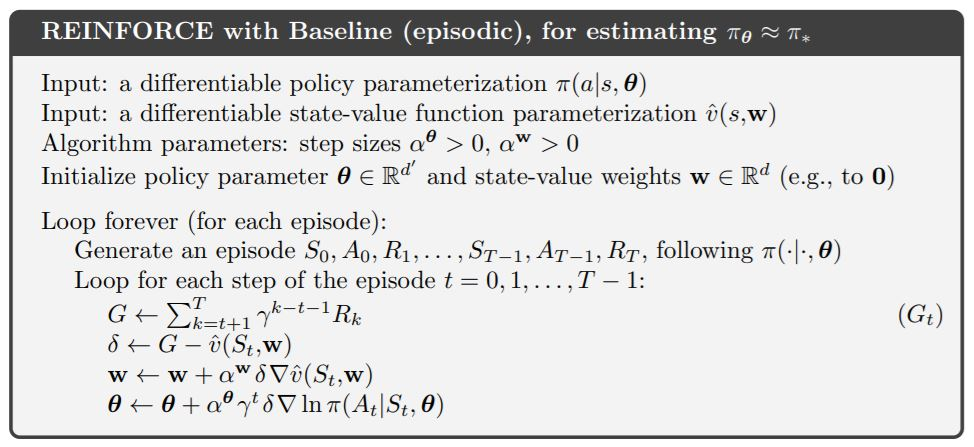
\includegraphics[width=.9\linewidth]{reinforcement_learning/reinforce_baseline.jpg}\end{center}


\subsection{actor-critic}
REINFORCE has no bias because it relies on sample returns, but it can suffer from high variance. We can reduce the variance (while introducing bias) by constructing bootstrapped targets, e.g. by replacing $G_t$ with a one-step TD target:

$$ \theta_{t+1} = \theta + \alpha \left[R_{t+1} + \gamma \hat{v}(S_{t+1}) - \hat{v}(S_t) \right] \nabla \ln \pi (A_t \mid S_t)$$

Here the \textit{critic} learns the value function and the \textit{actor} learns to update the policy to increase future reward.  

\subsection{policy parameterizations}
Policy gradient methods present a natural way of dealing with large or continuous action spaces. Rather than learning probability mass functions over many different actions, we can directly learn the parameters of probability distributions, for example the mean and standard deviation of gaussians in action space.
